\section{Experiments}
%\subsection{Experimental Setup}
%\textbf{Dataset and Evaluation Methodology}.
Our experiments are designed to answer: 1) whether it is possible to automatically collect training data for event extraction, 2) whether
extractors trained on such data can detect events of interest and identify their corresponding arguments, and 3) whether our solution can
work with other knowledge resources for more types of event.

 \subsection{Dataset Evaluation}\label{sec:evalhypo}
We start by comparing key argument selection strategies: %different data-collecting strategies:
(1) \emph{ALL}: uses all arguments as key arguments; (2) \emph{IMP}: uses the top half arguments with highest importance scores as key
arguments;
%we select the top half arguments with highest importance values as key arguments;
(3) \emph{IMP\&TIME}:  includes a time-related argument together with  the arguments selected by \emph{IMP};
and (4) \emph{DIS}: eliminate sentences where the dependency distances
 between any two key arguments are greater than 2.
%(3) \emph{IMP\&TIME} means adding a time-related argument with the highest importance value to %the set of key arguments defined by
%\emph{IMP}; (4) \emph{DIS}: we eliminate sentences where the dependency distances between any two key arguments are greater than 2.
We use the above methods to collect datasets using Freebase and the English Wikipedia dump of 2016-11-20, by randomly selecting 100
sentences from each dataset, and ask two annotators to decide if each sentence implies a given event type.



%To investigate the possibility of automatically constructing training data for event extraction,

As shown in Table~\ref{tab:3}, it is not surprising that \emph{ALL}, as the most strict, guarantees the quality of the collected data, but only contributes 203 sentences covering 9 event types, which is far from sufficient for further applications. \emph{IMP} relaxes \emph{ALL} by allowing the absence of non-key arguments, which expands the resulting dataset, but introduces more noise.
We can also see that the dependency constraint (DIS) improves the data quality (\emph{IMP}+\emph{DIS}).
%indicating that \emph{T2} is inappropriate to be used as a soft constraint.
Compared with \emph{IMP}, the significant quality improvement by \emph{IMP\&TIME} proves that time-related arguments within CVT schemas are critical to imply an event occurrence. Among all strategies, the dataset by \emph{IMP\&TIME}+\emph{DIS}  achieves the best quality, while still accounting for 46735 sentences with 50109 events, almost 10 times more than the ACE dataset, showing that it is feasible to automatically collect quality training data for event extraction without either human-designed event schemas or \textbf{extra} human annotations.
% our hypothesis \emph{H3} and \emph{H4} are feasible and it is an effective way to generate reliable data automatically.

Our final dataset, \textbf{FBWiki}, using \emph{IMP\&TIME}+\emph{DIS} , contains 46,735 positive sentences and 79,536 negative ones\footnote{Besides trivial negative samples that have no matched arguments, we randomly sample 34,837 negative instances that contain only part of key arguments, and 21,866 sentences whose key arguments violate the dependency constraint.}
 a random split of 101,019 for
training and 25,252 for testing. There are on average 4.8 arguments per event, and in total, 5.5\% instances labeled with more than two
types of events.


\begin{table}[t!]
\scriptsize
\centering
\begin{tabular}{lccc}
     \toprule
	 \textbf{Strategy} & \textbf{Sentences} & \textbf{Type} & \textbf{Positive Percentage (\%)} \\
     \midrule
	 \rowcolor{Gray}\emph{ALL} & 203 & 9 & 98\% \\
	 \emph{IMP} & 318K & 24 & 22\% \\
	 \rowcolor{Gray} \emph{IMP}+\emph{DIS} & 170K & 24 & 37\% \\
	 \emph{IMP\&TIME} & 112K & 24 & 83\% \\
	 \rowcolor{Gray} \emph{IMP\&TIME}+\emph{DIS} & 46K & 24 & 91\% \\
     \bottomrule
\end{tabular}
\vspace{-2mm}
\caption{Statistics of the datasets built with different strategies.
% \textit{Instances} denotes the number of CVT instances that can be used for each hypothesis.
%\textit{Sent.} is the number of sentences found.
\textit{Type} the number of different CVT types found.
%\textit{Positive} is the percentage of sentences mentioning the given events explicitly.
\label{tab:3}}
\vspace{-3mm}
\end{table}


%Statistics for the generated dataset from Freebase is shown in Table~\ref{statistics}.

%\begin{table}
%\small
%\centering
%\begin{tabular}{|l|c|c|c|} \hline
%& Train & Dev & Test \\ \hline
%\emph{\#PosSent.} & 29912 & 7477 & 9346 \\ \hline
%\emph{\#NegSent.} & 50904 & 12726 & 15906  \\ \hline
%\emph{\#Eve.} &  &  &  \\ \hline
%\emph{\#Arg.} &  &  &  \\ \hline
%\emph{\%Multi\_Eve.} &  &  &  \\ \hline
%\end{tabular}
%\caption{Statistics for the generated dataset. \emph{\#PosSent.} is the number of positive sentences, \emph{\#NegSent.} is the number of positive sentences, \emph{\#Eve.} is the number of event mentions, and \emph{\#Arg.} is the number of event arguments. \emph{\%Multi\_Eve.} is the ratio of multi-type events.
%, and \emph{\%Multi\_Arg.} is the ratio of multi-word arguments.
%\label{statistics}}
%\end{table}

%%%% containing 7,180 sentences, containing 7,394 events and 25,840 arguments. We then randomly select 4,800 sentences for training and 1,180 sentences as test set, and the rest 1,200 sentences for validation.
%We first manually evaluate the quality of our test set and then regard the automatically generated data as gold standard and evaluate our model accordingly. Next, we manually evaluate a subset of events detected by our model and analyze the differences with regards to the automatic evaluation. Finally, we conduct evaluation on a smaller dataset constructed according to Wikipedia tables and articles.
\vspace{2mm}

\noindent\textbf{\emph{Trigger Inference}: \mbox{ }} To further explore the relationship between key arguments and triggers, we regard the
least common ancestor of all key arguments in the dependency tree as a trigger candidate. As listed in Table~\ref{freqTriggers}, these
candidates share similar meanings and are highly informative to the underlying event types, showing that our key arguments with necessary
constraints can play the same role with explicit triggers in identifying an event.
% Although missing explicit information from \KB, most triggers can be inferred from the dependencies between a group of key arguments and its context.

\begin{table}
	\scriptsize
	\centering
	\begin{tabular}{lll}
    \toprule
		\textbf{Event types} & \textbf{Trigger candidates} & \textbf{Percentage} \\
    \midrule
		\rowcolor{Gray}film\_performance & play, appear, star, cast, portray & 0.72 \\
		award\_honor & win, receive, award, share, earn & 0.91 \\
		\rowcolor{Gray}education & graduate, receive, attend, obtain, study & 0.83 \\
		acquisition & acquire, purchase, buy, merge, sell & 0.81 \\
		\rowcolor{Gray}employ.tenure & be, join, become, serve, appoint & 0.79 \\
    \bottomrule
	\end{tabular}
    \vspace{-2mm}
	\caption{Top 5 most frequent trigger candidates and their proportions over all positive instances within each type.}
    \vspace{-3mm}
	\label{freqTriggers}
\end{table}

\vspace{2mm} \noindent\textbf{\emph{On ACE}: \mbox{ }} We also test our strategy on the ACE dataset. We first collect all annotated events,
without triggers, as the knowledge base to compute the importance values for all arguments, and select the key arguments for each ACE event
type accordingly. We follow \emph{IMP\&TIME}+\emph{DIS} to examine every sentence whether it can be selected as an annotated instance
within the ACE event types. Eventually, we correctly obtain 3,448 sentences as positive instances, covering 64.7\% of the original ACE
dataset.  We find that the main reason for the missing 35.3\% is that many arguments in the ACE dataset are pronouns, where our strategy is
currently unable to treat pronouns as key arguments. However, if a high-precision coreference resolution tool is available to preprocess
the document,
our solution would be able to automatically label more instances.% as training data.
% \textbf{ANYTHING NOVEL that traditional ACE does not have??? multple types? multiple events?}

 \subsection{Extraction Setup}\label{sec:evalevent}
Next, we evaluate our event extractor on FBWiki  %the collected datasets,
%\paragraph{Metrics:} We evaluate our models
%in terms of popular metrics in event extraction, i.e.,
with \emph{precision} (P), \emph{recall} (R), and \emph{F-measure} (F) for each subtask. These metrics are computed according to the
following standards of correctness. For \emph{event classification}, an event is correctly classified if its reference sentence contains
\textbf{all key arguments} of this event type. For \emph{key argument detection}, an event is correctly detected if its type and all of its
key arguments match a reference event within the same sentence. For \emph{all argument detection}, an event is correctly extracted if its
type and all of its arguments match a reference event within the same sentence.

\vspace{2mm}


\noindent \textbf{\emph{Training}:} All hyper-parameters are tuned on a development split in the training set. During event detection, we
set the size of word embeddings to 200, the size of LSTM layer to 100. In argument detection, we use the same size of word embedding, while
the size of LSTM layer is 150, and the size of key argument embedding is 50. Word embeddings are pre-trained using skip-gram
word2vec~\cite{mikolov2013distributed} on English Wikipedia and fine tuned during training. We apply dropout (0.5) on both input and output
layers.




\vspace{2mm}\noindent\textbf{\emph{Baselines}:}
%To investigate the effectiveness of our proposed model,
We compare our proposed model with three baselines.
The first is a  BLSTM model that takes word embeddings as input, and outputs the label for each word with the maximum probability. % among all possible labels.
For feature-based methods, we apply CRF (using the CRF++ toolkit~\cite{kudo2005crf++} ) and Maximum Entropy \cite{berger1996maximum} (Le
Zhang's MaxEnt toolkit) to explore a variety of elaborate features, according to the state-of-art feature-based ACE event
extractors~\cite{li2013joint}. Note that after key argument detection, we add the resulting label of each word as a supplementary feature
to detect non-key arguments.

\subsection{Compare with Automatic Annotations}
Firstly, we compare the model output against the automatically obtained event annotations.
As shown in Table~\ref{tab:1}, feature-based models perform worst in both event classification and argument detection.
One of the main reasons is the absence of explicit trigger annotations in our dataset, which makes it impossible to include trigger-related features, e.g., trigger-related dependency and position features.
Although traditional models can achieve higher precisions, they only identify a limited number of events, resulting in low recalls.
Neural-network methods perform much better than feature-based models, especially in recall, since they can make better use of word semantic features. Specifically, BLSTM can capture longer dependencies and richer contextual information, instead of neighbouring word features only.
The CRF layer brings an averagely 2\% improvement in all metrics, and by adding the ILP-based post inference, our full model, BLSTM-CRF-ILP$_{multi}$, achieves the best performance among all models.
% Moreover, neural-network-based methods can avoid errors propagating from other NLP preprocessing tools like POS tagging and NER.

\begin{table*}[!t]
\centering
\scriptsize
\begin{tabular}{|l|p{1.cm}<{\centering}|p{1.cm}<{\centering}|p{1.cm}<{\centering}|p{1.cm}<{\centering}|p{1.cm}<{\centering}|p{1.cm}<{\centering}|p{1.cm}<{\centering}|p{1.cm}<{\centering}|p{1.cm}<{\centering}|} \hline
	\multirow{2}{*}{\textbf{Model}} & \multicolumn{3}{c|}{\textbf{Event Type}} & \multicolumn{3}{c|}{\textbf{Key Argument Detection}} &
	\multicolumn{3}{c|}{\textbf{All Argument Detection}} \\ \cline{2-10}
	 & \textbf{P} & \textbf{R} & \textbf{F} & \textbf{P} & \textbf{R} & \textbf{F} & \textbf{P} & \textbf{R} & \textbf{F }\\ \hline
	\rowcolor{Gray} CRF & 88.9 & 11.0 & 19.6 & 36.1 & 4.47 & 7.96 & 19.9 & 3.06 & 5.30  \\ \hline
	MaxEnt & \textbf{95.2} & 12.4 & 21.9 & 41.6 & 5.40 & 9.56 & 22.5 & 3.40 & 5.91 \\ \hline
	\rowcolor{Gray} BLSTM & 89.8 & 63.0 & 74.1 & \textbf{64.9} & 45.5 & 53.5 & 42.9 & 27.7 & 33.7  \\ \hline \hline
	BLSTM-CRF & 86.4 & 67.4 & 75.7 & 63.6 & 49.6 & 55.8 & \textbf{44.4} & 31.0 & 36.5  \\ \hline
	\rowcolor{Gray} BLSTM-CRF-ILP$_{1}$ & 84.4 & 74.1 & 78.9 & 62.3 & 53.8 & 57.3 & 42.7 & 33.8 & 37.7 \\ \hline
	BLSTM-CRF-ILP$_{multi}$ & 85.3 & \textbf{79.9} & \textbf{82.5} & 60.4 & \textbf{55.3} & \textbf{57.7} & 41.9 & \textbf{34.6} & \textbf{37.9} \\ \hline
\end{tabular}
\vspace{-2mm}
\caption{System performance when compared against automatic annotations (\%).  \label{tab:1}}
\vspace{-3mm}
\end{table*}

% \paragraph{Multi-word Argument Detection}
% Committing to the multi-word argument issue, we treat each subtask as a sequence labeling problem. Evaluated on multi-word arguments, the F1 scores of BLSTM-CRF, BLSTM-CRF-ILP$_1$ and BLSTM-CRF-ILP$_{multi}$ in argument detection are 71.3\%, 80.5\%, and 81.0\%, respectively.

%\paragraph{The CRF Layer:}
%As seen in Table~\ref{tab:1},
It is not surprising that  every model with a CRF layer over its BLSTM layer is superior to the one with a BLSTM layer only. Compared with vanilla BLSTM, BLSTM-CRF achieves higher precisions and recalls in all subtasks by significantly reducing the invalid labelling sequences (e.g., \texttt{I-arg} appears right after \texttt{O}). During prediction, instead of tagging each token independently, BLSTM-CRF takes into account the constraints between neighbouring labels, and potentially increases the co-occurrences of key arguments regarding the same event type. % in some way.

%\paragraph{The ILP Post Inference:}
As shown in Table~\ref{tab:1}, the ILP-based post inference considerably improves the overall performance, especially in \textit{event type classification}. With the help of constraint \textbf{C4},  dubious key arguments can be correctly inferred through other key arguments from their context. Compared with BLSTM-CRF, BLSTM-CRF-ILP$_1$ produces an F1 gain of 3.2\% in event type classification, 1.5\% in key argument detection, and 1.2\% in all argument detection. %, with respect to tF1.

\vspace{2mm}\noindent\textbf{\emph{Multi-type Events}:}
%We further investigate the effect of
Among all methods, BLSTM-CRF-ILP$_{multi}$ is the only model that can deal with multi-type event mentions. %As shown in Table~\ref{tab:1},
The proposed strategy ILP$_{multi}$ helps detect more event mentions for a sentence, contributing to the increase of recalls, and F1 scores with a little drop of precisions.
%\textbf{Evaluated on \textbf{38XXXX} sentences containing multi-type event mentions, the F1 scores of BLSTM-CRF-ILP$_{multi}$ in event type classification, event detection and argument detection are 70.7\%, 58.4\% and 26.9\%, respectively.}
BLSTM-CRF-ILP$_{multi}$ can correctly identify 132 sentences with multi-type events,
with an accuracy of 95.6\%, and for each involved event, our model maintains a high
performance in identifying its arguments, achieving 45.5\%, and 29.1\% in F1 for key argument detection and all argument detection, respectively.

\subsection{Manual Evaluation}\label{manualeve}
To provide a deep investigation about our dataset and models, we randomly sample 150 sentences from the test set. Two annotators are asked
to annotate each sentence following two steps. First, determine if a given sentence is positive or negative, and assign \textbf{all
possible} event types to positive ones. Next, label all related arguments and their roles according to the event types for all positive
instances. Two annotators will independently annotate each sentence, and discuss to reach an agreement. The inter-annotator agreement is
87\% for event types and 79\% for arguments.


By comparing the automatic and manual annotations on the 150 sentences, we find that the main issue for the automatic annotation is that
some automatically labeled sentences do not imply any event while still matching all key properties of certain \CVT entries in Freebase. We
find 16 such instances that are mistakenly labeled as positive. For example in Figure~\ref{fig:1}, although the phrase \underline{\emph{the
car}} in S6 matches a film name, it does not refer to a film. This is because that we currently do not have a strong entity linker to
verify those entities, which we leave for future work. However, during manual investigation, BLSTM-CRF-ILP$_{multi}$ can correctly identify
these 6 instances as negative.


%\begin{table}[h]
%\scriptsize
%\centering
%\begin{tabular}{|l|p{0.8cm}<{\centering}|p{0.8cm}<{\centering}|p{0.8cm}<{\centering}|} \hline
%	% Model & EC & AD & ED \\ \hline
%	% CRF & 21.2 & 13.3 & 5.30 \\ \hline
%	% MaxEnt & 17.7 & 11.7 & 5.44 \\ \hline
%	% BLSTM & 79.8 & 64.3 & 41.2 \\ \hline \hline
%	Model & EC & KAD & AAD \\ \hline
%	BLSTM-CRF & 75.4 & 54.7 & 35.5 \\ \hline
%	BLSTM-CRF-ILP$_{1}$ & 77.2 & 56.1 & 35.7 \\ \hline
%	BLSTM-CRF-ILP$_{multi}$ & \textbf{80.7} & \textbf{56.4} & \textbf{36.3} \\ \hline
%\end{tabular}
%\caption{The F1 scores of different systems on the manually annotated data. EC, KAD, AAD denote the event type classification, key argument detection and all key argument detection, respectively. \label{tab:2}}
%\end{table}

On this manually annotated dataset, we can observe similar trends with Table~\ref{tab:1}, and BLSTM-CRF-ILP$_{multi}$ remains the best performing model, achieving 80.7\%, 56.4\% and 36.3\% in F1 scores for event type, key argument detection and all argument detection, respectively.
%where we can observe similar trends with Table~\ref{tab:1}, that
%both CRF layer and ILP$_{multi}$ greatly improve the overall performance and

%Table~\ref{tab:2} summarizes the performances of different models on the manually annotated dataset, where we can observe similar trends with Table~\ref{tab:1}, that
%both CRF layer and ILP$_{multi}$ greatly improve the overall performance and
% shows the system performances in the manual evaluation. We can draw similar conclusions about the comparison of performances between different models as automatic evaluation. It is clear that
%BLSTM-CRF-ILP$_{multi}$ remains the most effective model. %,  in event extraction as it achieves the highest F1 scores in both manual and automatic evaluation.

\begin{figure}[t!]
	\centering
	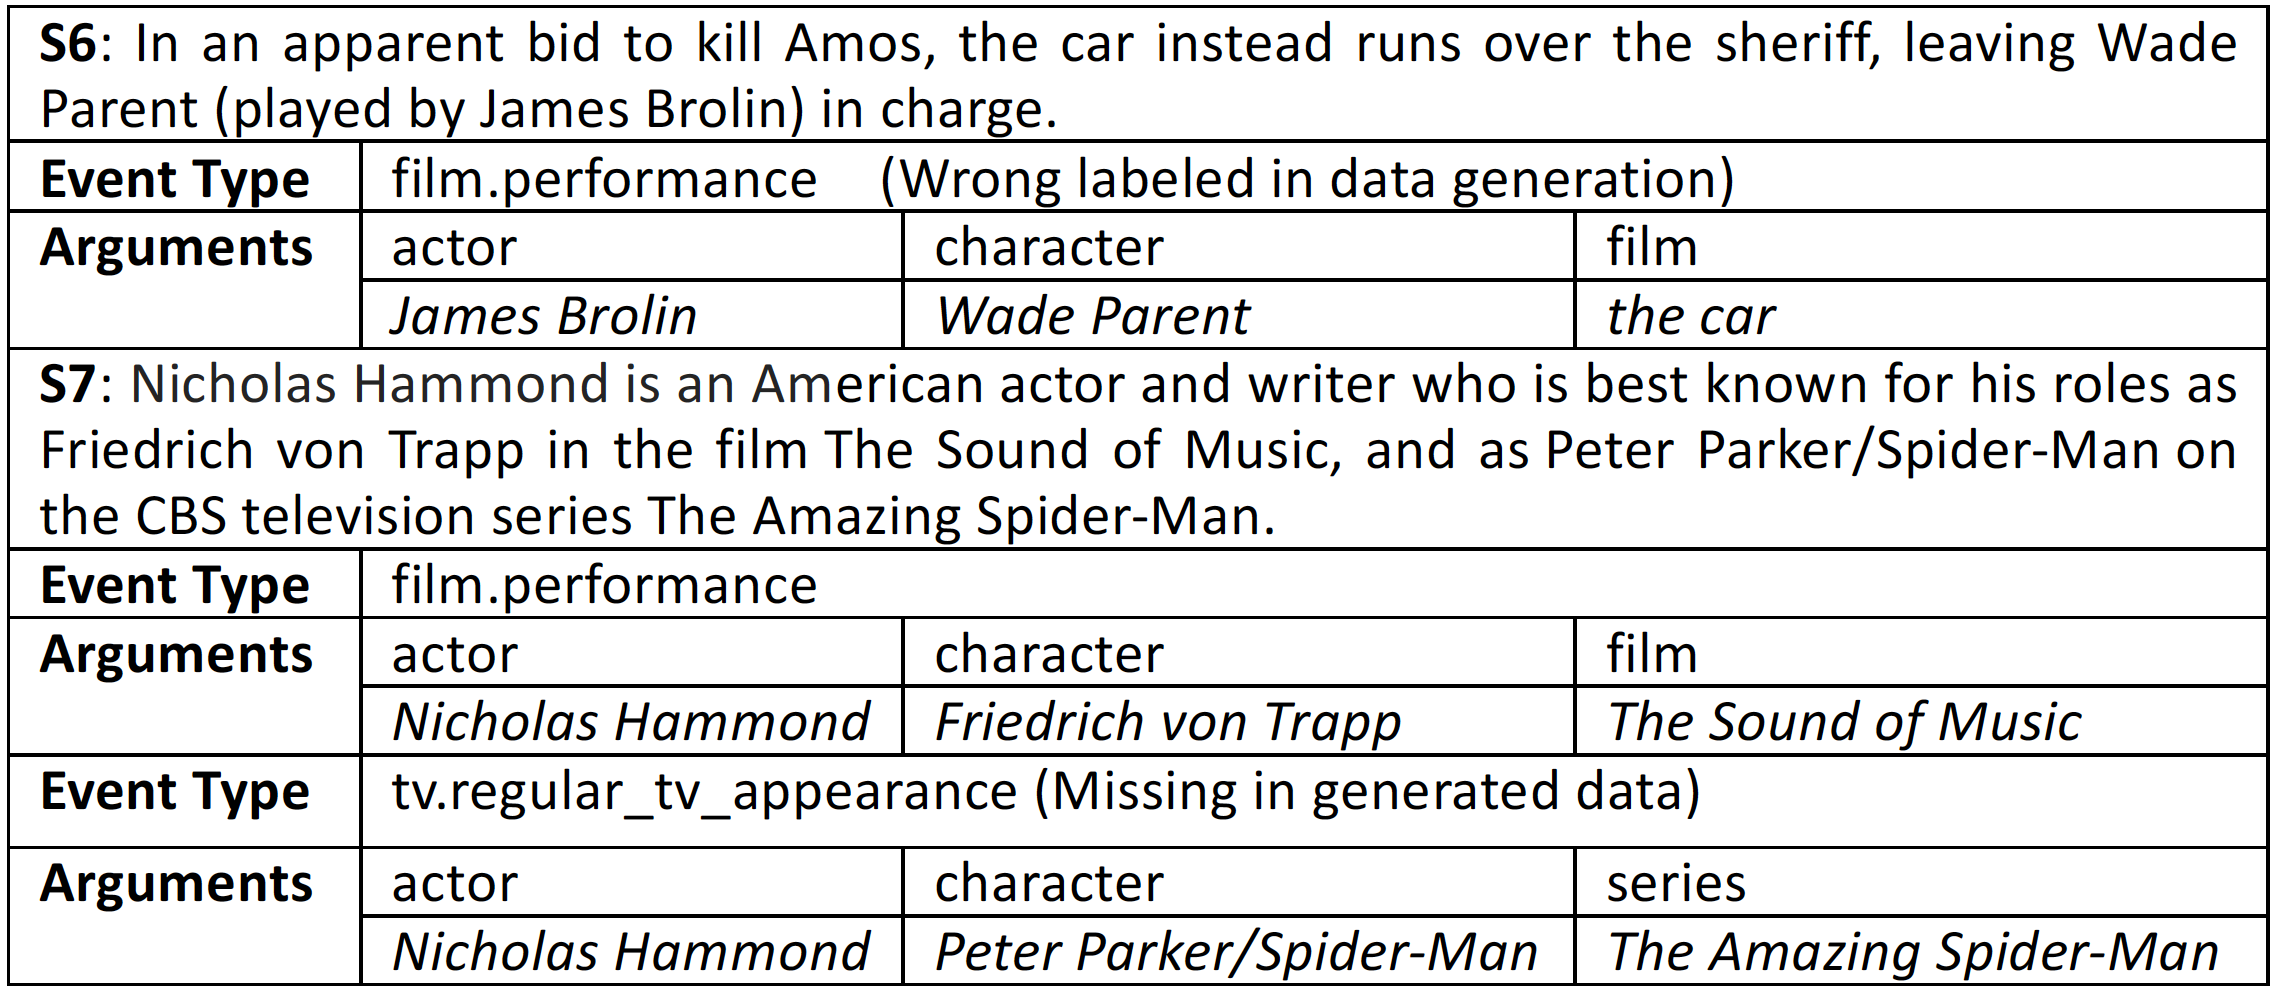
\includegraphics[width=.48\textwidth]{figure3(3).png}
    \vspace{-5mm}
	\caption{Example outputs of BLSTM-CRF-ILP$_{multi}$.\label{fig:1}}
    \vspace{-5mm}
\end{figure}



%Moreover, %manual evaluation may help us to gain a deep insight about our data and models. We
% we manually check the top 5 event types whose EC F1 scores by BLSTM-CRF-ILP$_{multi}$ differ greatly between automatic evaluation and manual evaluation, summarized in Table~\ref{tab:4}. We find that most of the performance differences are caused by data generation. Figure~\ref{fig:1} examples two types of errors in data construction. Several automatically labeled sentences do not imply any event while still matching all key properties of some CVT entries. For example, although the phrase \emph{the car} in S5 matches a film name, it does not indicate this film, and there is no explicit evidence indicating that an actor starred in this film. This is a bottleneck of our data generation strategy. During manual evaluation, we find 16 negative sentences which are mistakenly labeled as positive, and our model manages to rectify 6 of them.

Remarkably, our BLSTM-CRF-ILP$_{multi}$ model can find more \CVT instances that are currently not referenced in Freebase. Our model detects two events in S7, while the arguments of the \textit{tv.tv\_appearance} event do not match any existing CVT instances in Freebase, which do not receive any credit during automatic evaluation, but should be populated into Freebase. %leading to a missing event in data generation.
This  suggests that by learning from distant supervision provided by Freebase, our model can be used to populate or update Freebase instances in return.

%\begin{table}[h]
%\small
%\centering
%\begin{tabular}{|l|c|c|c|} \hline
%	Event type & P & R & F \\ \hline
%	olympics.medal\_honor%\footnote{The full name is olympics.olympic\_medal\_honor in Freebase.}
%	& $\downarrow$ 25.0\% & $\downarrow$ 5.0\% & $\downarrow$ 13.8\% \\ \hline
%	film.performance & $\downarrow$ 21.4\% & $\uparrow$ 3.1\% & $\downarrow$10.3\% \\ \hline
%	business.acquisition & $\rightarrow$ & $\downarrow$ 7.1\% & $\downarrow$ 5.4\% \\ \hline
%	tv.appearance%\footnote{The full name is tv.regular\_tv\_appearance in Freebase.}
%	& $\downarrow$ 9.5\% & $\uparrow$ 3.0\% & $\downarrow$ 3.1\% \\ \hline
%	film.release%\footnote{The full name is film.film\_regional\_release\_date in Freebase.}
%	& $\downarrow$ 7.7\% & $\uparrow$ 5.6\% & $\downarrow$ 0.55\% \\ \hline
%\end{tabular}
%\caption{The difference of EC F1 scores (by BLSTM-CRF-ILP$_{multi}$) between automatic and manual evaluation for top 5 event types.\label{tab:4}}
%\end{table}

\vspace{2mm}\noindent\textbf{\emph{On BBC News}:}
% 在BBC新闻上抽取business.acquisition和tv.regular_tv_appearance两类事件,并用规则更新
We further apply our event extractor, trained on FBWiki, to 397 BBC News
articles (2017/04/18 -- 2017/05/18 in Politics, Business and TV sections), and manually examine the extraction results. We find that our model is able to correctly identify 117 events, and 53 events,
almost half of which are not covered in the currently used Freebase.



\subsection{Tables as Indirect Supervision}
To investigate the applicability of our approach to other structured knowledge/tables besides Freebase \CVT tables, we automatically build
a new dataset, \textbf{TBWiki}, with the supervision provided by Wikipedia tables, which characterize events about business acquisition,
winning of the Olympics games, and awards winning in entertainment (Table~\ref{tab:6}).

\begin{table}[t]
\scriptsize
\centering
\begin{tabular}{lccccc}
    \toprule
	\textbf{Event type} & \textbf{Entries} & \textbf{Positive} & \textbf{EC} & \textbf{KAD} & \textbf{AAD} \\
    \midrule
	\rowcolor{Gray} Acquisition & 690 & 414 & 87.0\% & 72.0\% & 69.6\% \\
	Olympics & 2503 & 1460 & 77.2\% & 64.5\% & 38.6\% \\
	\rowcolor{Gray} Awards & 3039 & 2217 & 95.0\% & 82.8\% & 58.6\% \\
    \bottomrule
\end{tabular}
\vspace{-2mm}
\caption{Statistics of the TBWiki dataset and the performance (in F1) of our model on TBWiki.
%\textit{Entr.} is the number of table entries. \textit{Sent.} is number of positive instances.
EC, KAD and AAD denote event type classification, key argument detection and all key argument detection, respectively.
\label{tab:6}}
\vspace{-5mm}
\end{table}

We train our BLSTM-CRF-ILP$_{multi}$ on this dataset and evaluate it on 100 manually annotated sentences.
% and follow the same steps of event annotations as mentioned in Section~\ref{manualeve}.
We can see that without extra human annotations, %Table~\ref{tab:6} demonstrates that tabular data as distant supervision can be adapted to extract high-confidence events
our model can learn to extract events from the training data weakly supervised by Wikipedia tables. Given a specific event type, as long as we can acquire tables implying events of such type, it is possible to automatically collect training data from such tables, and learn to extract structured event representations of that type. % an effective but robust event extractor. , which is much easier than human annotation and unlimited in event types.
